Network-based approaches to cognitive neuroscience typically assume that mental representations are encoded as distributed patterns of activation over large neural populations, with different populations encoding different kinds of representational structure and communicating this structure to other network components. Extensive research over the past several years has focused on testing such hypotheses using data from functional brain imaging techniques such as fMRI. The best-known approach in this vein has been \emph{Representational Similarity Analysis} (RSA) \cite{RSA}, which seeks to discover brain regions whose activity encodes the known psychophysical similarities among some set of stimuli. RSA is typically applied either to a specific brain region of interest (ROI) or across the whole brain via {\em searchlight analysis} \cite{searchlight}, which applied the technique to many small spherical clusters throughout the measured volume. For each such region the cosine distances between vectors of evoked responses are computed for all stimulus pairs, and the resulting neural dissimilarity matrix is correlated with the target matrix that expresses psychophysical distances of interest amongst the stimuli. If these correlations are reliably non-zero, this suggests the corresponding region may encode the similarity information.

A drawback of ROI and searchlight RSA is that these methods place strong assumptions on the anatomical structure of the regions thought to encode the similarities of interest (predefined ROIs or spherical clusters). In this paper we propose a new approach for {\em whole-brain} RSA that can discover arbitrarily structured brain networks (possibly widely
distributed and non-local) that encode similarity information. The key insight behind our method is that RSA can be posed as a multi-task regression problem which, in conjunction with sparsity regularization methods, can automatically detect networks of voxels that appear to jointly encode similarity information.

Our new approach, called Network RSA (NRSA), is summarized as follows (see Sections~\ref{wbrsa1}~and~\ref{wbrsa2} for further details).  Consider a set of $n$ items and suppose we are given an $n \times n$ similarity matrix $\bS$, where the $ij$-th element $\bS_{ij}$ is the similarity\cite{similarity} between item $i$ and item $j$. For example, these may come from human judgments of perceptual similarity between pairs of stimuli.  RSA is based on the hypothesis that there exists a set of voxels whose correlations encode the similarities in $\bS$, as depicted in Figure~\ref{fig.fitting}.


\begin{figure}[!h]
	\centering
	          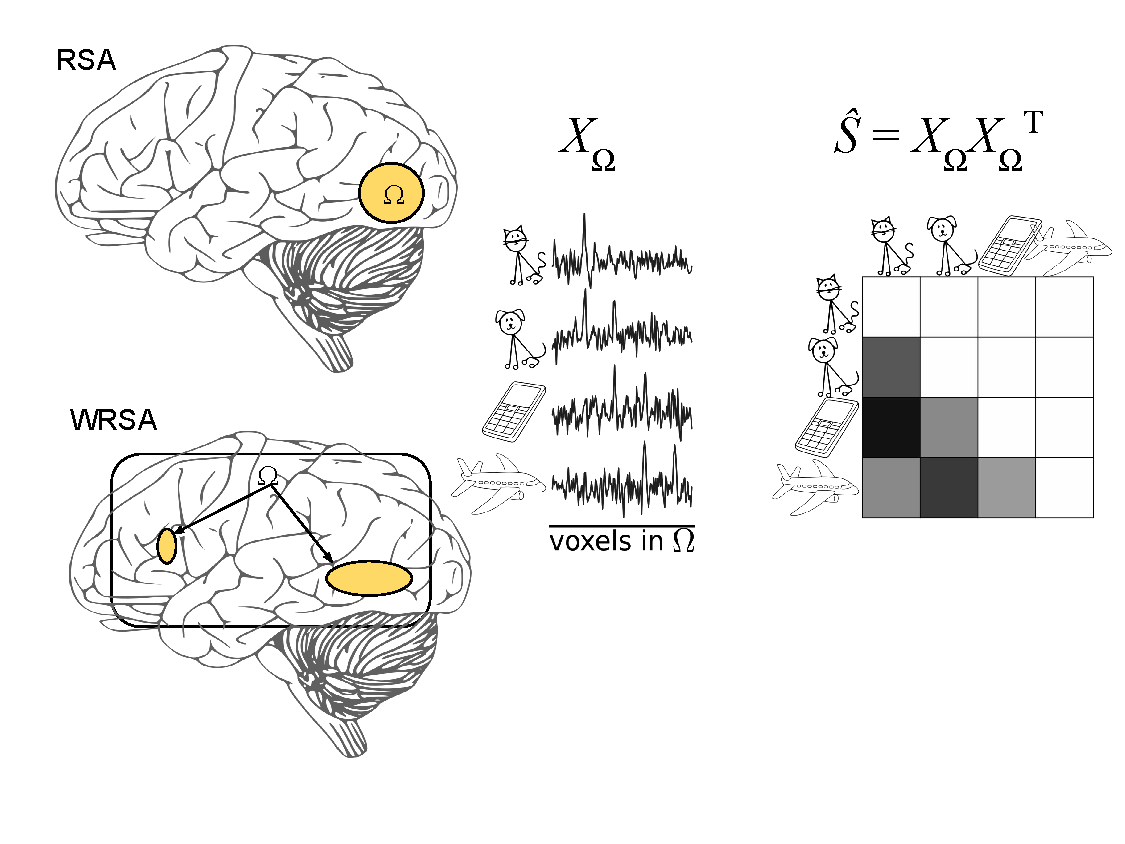
\includegraphics[width=0.5\textwidth]{figures/WRSA.pdf} \\
	        
	\caption{Representational Similarity Analysis.  Traditional RSA methods consider only localized brain networks, such as specific regions of interest or spherical clusters of the cortex (upper left) \cite{RSA,searchlight}.  We propose a new {\em Network} RSA (NRSA) method that can potentially identify non-local brain networks that encode similarity information (lower left).  Within a set of voxels $\Omega$ (localized or non-local), the correlations between the activation patterns resulting from different stimuli approximate (perceptual) similarities between the stimuli.  } \label{Fig:WRSA}
	\label{fig.fitting}
\end{figure}


Let $\bX \in \R^{n\times p}$ denote a matrix of voxel activations.
Each row corresponds activations in all $p$ voxels in response to a specific stimulus, and each column corresponds to the activations in specific voxel to the $n$ different stimuli.  Our generalized notion of RSA,
which encompasses conventional ROI \cite{RSA} and searchlight \cite{searchlight} approaches, involves finding a sparse symmetric positive semi-definite matrix  $\bW\in \R^{p\times p}$ such that
$$\bS \ \approx \bX \bW \bX^T \ .$$
%We call $\bX\bW\bX^T$ a similarity representation.
By sparse we mean that at most $k<p$ rows/columns of $\bW$ are nonzero.   The locations of the nonzero elements indicate which voxels are included in the similarity-encoding brain network, and the  weights in $\bW$ indicate the strength of the edges in the network.  For instance, consider the $n\times 1$ activation vectors of two voxels $\bx_k$ and $\bx_{\ell}$ (i.e., the $k$th and $\ell$th columns of $\bX$).  It is easy to show that the contribution of these two voxels to the similarity representation is given by $ W_{k,\ell} \, \bx_k \bx_{\ell}^T + W_{\ell,k} \, \bx_\ell \bx_{k}^T$.  If $W_{k,\ell}=W_{\ell,k}\neq 0$, then the correlations between the two voxels contribute to the approximation of the similarity matrix $\bS$. The complete similarity representation can be expressed as
$$\bS \ \approx \ \bX\bW\bX^T \ = \ \sum_{k,\ell=1}^p W_{k,\ell} \, \bx_k \bx_{\ell}^T + W_{\ell,k} \, \bx_\ell \bx_{k}^T  \ .$$
The approximation problem can be posed as the least squares optimization
$$\min_{\bW} \|\bS-\bX\bW\bX^T\|_F^2 \ , $$
where the objective is the Frobenius norm of the difference between the similarity matrix $\bS$ and its approximation in terms of voxel activations.  If the number of voxels $p$ exceeds the number of items $n$ (which is usually the case in whole-brain RSA), then the system of equations is underdetermined and there will be many solutions to the optimization above.  Moreover, the hypothesis underlying RSA is that a small subset of the brain encodes the similarity representations.  To account for this,
the optimizations can be modified by including regularizer terms that encourage sparse solutions, as discussed in the next section.



\section{Learning Similarity Encodings \\ via Group Lasso}


Throughout the paper, we will assume that the similarity matrix $\bS$ is symmetric and positive-semidefinite (PSD) and is exactly or approximately low-rank.  Since $\bS$ is known, its low-rank structure can be determined from its singular value decomposition. Similarity matrices are often low-rank because of clustering or other relationships between the items under consideration. For example, in our experimental application described later in the paper, we find that a rank $r=3$ approximation is quite accurate.  Since we suppose that the given similarity matrix $\bS$ may be (approximately) low-rank, this suggests the convex optimization
$$\min_{\bW\in \S_+^p} \|\bS-\bX\bW\bX^T\|_F^2 \ + \ \lambda_1 \|\bW\|_\ast + \lambda_2 \|\bW\|_1 \ , $$
where $\S_+^p$ denotes the set of symmetric PSD $p\times p$ matrices, $ \|\bW\|_\ast$ is the nuclear norm of $\bW$, $\|\bW\|_1 $ denotes the $\ell_1$ norm of the elements in $\bW$, and $\lambda_1,\lambda_2>0$ are regularization parameters.  The nuclear norm encourages low-rank solutions and the $\ell_1$ term promotes solutions that include a small subset of the brain voxels. 
This type of optimization has been studied extensively \cite{maryam}.

Since $\bS \in \S_+^n$, we can work with the ``square-root" of $\bS$ instead (e.g., its Cholesky decomposition).  Suppose that $\bS$ has rank $r<n$ and let $\bY\in \R^{n\times r}$ satisfy $\bY\bY^T = \bS$ (or take $\bY$ corresponding to the best rank-$r$ approximation to $\bS$, given by the SVD). Consider the optimization
\begin{eqnarray}
\min_{\bB\in \R^{p\times r}} \|\bY-\bX\bB\|_F^2 \ .
\end{eqnarray}
This  optimization has the form of a multi-task regression \cite{obo11,lounici,vandegeer}, and a solution $\widehat \bB$ yields a weight matrix $\widehat \bW =  \widehat \bB \widehat\bB^{T}$.  Note that this optimization automatically enforces a rank $r$ solution, eliminating the need for the nuclear norm term above.
Although $\widehat \bW$ is not exactly a solution to the optimization $\min_{\bW} \|\bS-\bX\bW\bX^T\|_F^2$, it is easy to relate the two optimizations as follows.  Let $\widetilde \bW$ be a solution to $\min_{\bW} \|\bS-\bX\bW\bX^T\|_F^2$ and let $\widetilde \bB\widetilde\bB^T$ be its Cholesky factorization.
Assuming the normalization  $\|\widehat\bB\|_F, \|\widetilde \bB\|_F \leq 1$, we have
\begin{align*}
\|\widetilde \bW - \widehat{\bW} \|_F &= \|\widetilde \bB \widetilde\bB^{T} - \widehat{\bB} \widehat{\bB}^T\|_F\\
&\leq \|\widetilde \bB + \widehat{\bB} \|_F \|\widetilde \bB - \widehat{\bB}\|_F\\
&\leq (\|\widetilde\bB\|_F + \|\widehat{\bB}\|_F) \|\widetilde\bB - \widehat{\bB}\|_F\\
&\leq 2\|\widetilde\bB - \widehat{\bB}\|_F \ .
\end{align*}

The optimization $\min_{\bB\in \R^{p\times r}} \|\bY-\bX\bB\|_F^2$ can be modified to encourage sparse solutions by including a regularization term.
The most common approach to promote sparsity in multi-task regression is the group lasso:
\begin{equation}\label{eqn.grouplasso}
 \min_{\bB\in \R^{p\times r}} \|\bY-\bX\bB\|_F^2 \ + \ \lambda \|\bB\|_{1,2}  \ 
 \end{equation}
Here $\lambda>0$ is a regularization parameter and $ \|\bB\|_{1,2}$ is defined as follows.  The rows of $\bB$ are denoted by $\bbeta_{i \a}$, $i=1,\dots,n$, and the norm $\|\bB\|_{1,2} \ = \ \sum_{i=1}^n \|\bbeta_{i \a}\|_2$. This encourages solutions with only a few nonzero rows in $\bB$ \cite{obo11,lounici,vandegeer}.  

The main signal processing innovation in this paper is a new approach to the group lasso that is designed to cope with strongly correlated covariates (i.e., cases in which certain columns of $\bX$ may be close to, or even exactly, collinear).  This is a concern in fMRI, since certain voxels may have very correlated activation patterns.  In the standard (single-task) regression problem, this issue has been tackled using many techniques, including the elastic net \cite{EN}, OSCAR \cite{oscar} and OWL \cite{owl}, and others.  We propose a generalization of the recently proposed Ordered Weighted $\ell_1$ (OWL) approach to the multi-task setting, and thus call our new approach Group OWL (GrOWL).  

We show that GrOWL shares many of the desirable features of the OWL method, namely it automatically clusters and averages regression coefficients associated with strongly correlated columns of $\bX$.  This has two desirable effects, in terms of both model selection and prediction.  First, GrOWL can select all of the relevant voxels in $\bX$, unlike standard group lasso which may not select relevant voxels if they happen to be strongly correlated with others.  Second, GrOWL encourages the coefficients associated with strongly correlated voxels to be near or exactly equal.   In effect, this averages strongly correlated voxelss which can help to denoise activation patterns and improve predictions.  
